\chapter{Kết quả và thảo luận}

Trong chương này, em trình bày các kết quả thực nghiệm đạt được của phương pháp VRAE so với các phương pháp cơ sở (AE, GAN, FB). Các kết quả được đánh giá thông qua cả hai khía cạnh: định lượng (các chỉ số đo lường) và phân tích sâu về cơ chế hoạt động của mô hình.

\section{Đánh giá định lượng}

Hiệu suất của phương pháp đề xuất VRAE được so sánh với các mô hình GAN, FB và các biến thể của Autoencoder (AE) với các độ sâu khác nhau (từ 2 đến 5 khối). Kết quả chi tiết được tổng hợp trong Bảng \ref{tab:quantitative_comparison}.

\begin{table}[H]
\centering
\caption{So sánh định lượng giữa GAN, FB, AE và phương pháp VRAE đề xuất trên tập kiểm tra (Test set).}
\label{tab:quantitative_comparison}
\begin{tabular}{lccccc}
\hline
\textbf{Mô hình} & \textbf{PSNR (dB) $\uparrow$ } & \textbf{NMSE $\downarrow$ } & \textbf{SSIM $\uparrow$ } & \textbf{Tham số} & \textbf{FPS} \\ \hline
GAN (Gen) & 28,743 & 0,006 & 0,842 & 14,59M & 188 \\
FB (Gen) & 27,093 & 0,008 & 0,831 & 25,87M & 35 \\
AE2 & 27,787 & 0,007 & 0,840 & 0,375M & 411 \\
AE3 & 26,159 & 0,011 & 0,802 & 2,77M & 289 \\
AE4 & 29,404 & 0,005 & 0,864 & 14,59M & 189 \\
AE5 & 27,243 & 0,008 & 0,793 & 48,43M & 119 \\ \hline
VRAE2 & 30,319 & 0,004 & 0,884 & 0,376M & 399 \\
\textbf{VRAE3} & \textbf{31,052} & \textbf{0,003} & \textbf{0,898} & 2,78M & 194 \\
VRAE4 & 30,246 & 0,004 & 0,880 & 14,61M & 90 \\
VRAE5 & 30,032 & 0,003 & 0,860 & 48,48M & 45 \\ \hline
\end{tabular}
\end{table}

Dựa trên kết quả ở Bảng \ref{tab:quantitative_comparison}, có thể đưa ra các nhận xét sau:
\begin{itemize}
    \item \textbf{Độ chính xác tái tạo:} Mô hình \textbf{VRAE3} đạt kết quả cao nhất ở cả ba chỉ số PSNR (31,052 dB), SSIM (0,898) và có NMSE thấp nhất (0,003). Điều này khẳng định hiệu quả của cơ chế kết nối dọc (Vertical Residual) trong việc khôi phục chi tiết ảnh.
    \item \textbf{So sánh với AE truyền thống:} Khi so sánh ở cùng một độ sâu, VRAE luôn vượt trội hơn hẳn so với AE. Cụ thể, VRAE giúp cải thiện PSNR khoảng 20%, giảm NMSE xuống gần 50\% và tăng SSIM lên khoảng 1\% trong khi chỉ tăng một lượng rất nhỏ tham số (khoảng 1\%).
    \item \textbf{Hiệu năng tính toán:} Mô hình \textbf{VRAE2} cho thấy sự cân bằng tuyệt vời giữa chất lượng và tốc độ khi đạt 399 FPS, rất phù hợp cho các ứng dụng giám sát giao thông thời gian thực.
\end{itemize}

\section{Phân tích bảo toàn nội dung thông tin}

Để hiểu rõ hơn tại sao VRAE lại hoạt động hiệu quả, nghiên cứu thực hiện phân tích sự thay đổi Entropy giữa các lớp của bộ mã hóa. Entropy được dùng để đo lường lượng thông tin được giữ lại trong quá trình trích xuất đặc trưng.

\begin{figure}[H]
    \centering
    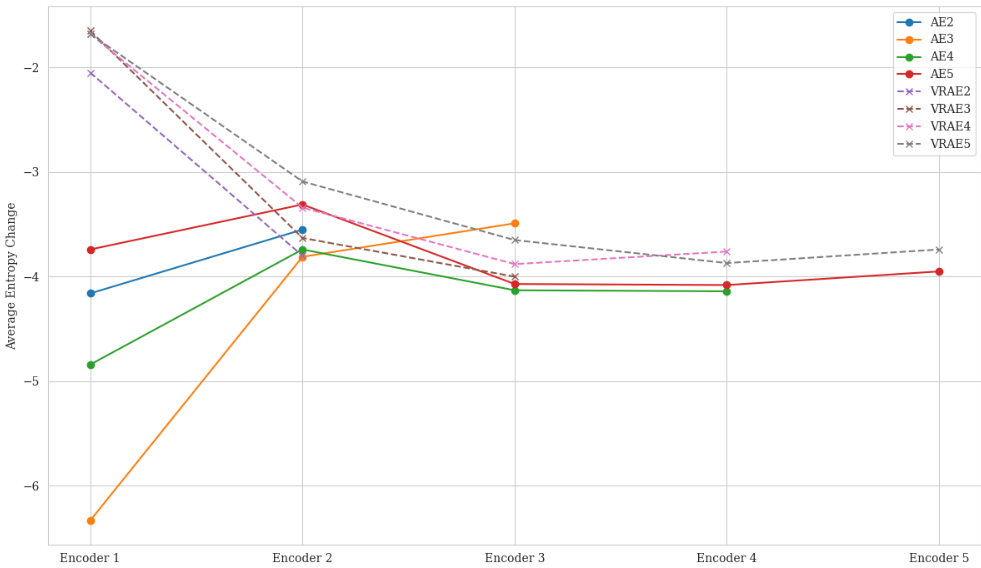
\includegraphics[width=0.8\linewidth]{images/entropy_change.png}
    \caption{Sự thay đổi Entropy trung bình qua các lớp mã hóa của AE và VRAE.}
    \label{fig:entropy_analysis}
\end{figure}

Kết quả phân tích cho thấy:
\begin{itemize}
    \item \textbf{Giai đoạn đầu:} Các mô hình VRAE bắt đầu với mức độ thay đổi Entropy cao hơn so với AE thông thường, đặc biệt là ở lớp mã hóa đầu tiên. Điều này chứng tỏ VRAE bảo toàn được nhiều đặc trưng thô và chi tiết vi mô hơn ngay từ đầu.
    \item \textbf{Sự ổn định:} Tốc độ giảm Entropy trong VRAE diễn ra mượt mà và nhất quán hơn so với AE. Ví dụ, VRAE3 giảm dần từ -1,5 xuống -3,7, trong khi AE3 giảm đột ngột từ -6,3 xuống -3,5. Sự thay đổi dần dần này giúp tránh hiện tượng "sụp đổ thông tin" (information collapse) quá sớm ở các tầng nông.
\end{itemize}

\section{Phân tích sự đánh đổi (Trade-offs)}

Thông qua phân tích mặt tiền Pareto (Pareto Front) giữa chất lượng tái tạo (PSNR/SSIM) và tốc độ suy luận (FPS), chúng em nhận thấy:

\begin{figure}[H]
    \centering
    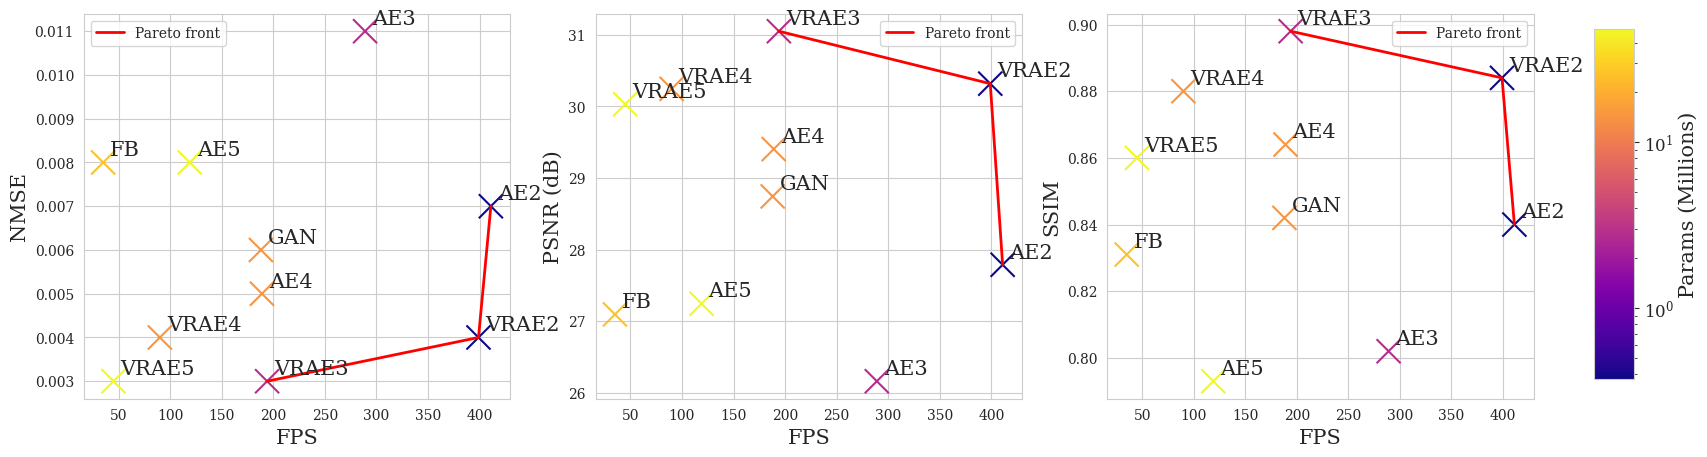
\includegraphics[width=1\linewidth]{images/pareto.png}
    \caption{Trực quan hóa sự đánh đổi giữa hiệu suất tái tạo (NMSE, PSNR, SSIM) và tốc độ suy luận (FPS) thông qua mặt tiền Pareto.}
    \label{fig:pareto_front}
\end{figure}

Chúng em nhận thấy:
\begin{itemize}
    \item Các biến thể VRAE (đặc biệt là VRAE2 và VRAE3) nằm trên đường biên tối ưu, thể hiện sự kết hợp tốt nhất giữa độ chính xác và hiệu năng.
    \item Ngược lại, các mô hình GAN và FB có số lượng tham số lớn nhưng hiệu quả tái tạo và tốc độ suy luận đều thấp hơn so với VRAE trong bài toán cụ thể này.
\end{itemize}



\section{Hướng phát triển trong tương lai}

Dựa trên những kết quả đạt được và các hạn chế còn tồn tại, nghiên cứu này có thể được mở rộng theo các hướng sau trong tương lai:
\begin{itemize}
    \item \textbf{Tối ưu hóa và nén mô hình:} Nghiên cứu các kỹ thuật nén mô hình như cắt tỉa (pruning), lượng tử hóa (quantization) và chưng cất tri thức (knowledge distillation). Các phương pháp này sẽ giúp giảm đáng kể dung lượng và tăng tốc độ suy luận, tạo điều kiện thuận lợi cho việc triển khai VRAE trên các thiết bị nhúng và hệ thống giám sát giao thông thực tế.
    \item \textbf{Kiến trúc độ sâu thích ứng:} Phát triển các khối mã hóa có khả năng tự động điều chỉnh độ sâu (adaptive-depth) tùy thuộc vào độ phức tạp của ảnh đầu vào, từ đó tiết kiệm tài nguyên tính toán cho những trường hợp ảnh ít nhiễu.
    \item \textbf{Khôi phục video thời gian thực:} Mở rộng phương pháp VRAE từ khôi phục ảnh tĩnh sang khôi phục luồng video, tận dụng thông tin liên quan giữa các khung hình kề nhau để tăng cường độ ổn định và chính xác của quá trình xử lý.
    \item \textbf{Đánh giá đa dạng:} Thực nghiệm mô hình trên nhiều bộ dữ liệu biển số xe khác nhau (như các loại biển số quốc tế, biển số xe máy) và trong các điều kiện thời tiết khắc nghiệt hơn (mưa lớn, sương mù dày đặc) để nâng cao tính tổng quát của nghiên cứu.
\end{itemize}

\section{Kết luận}

Trong chương này, em đã trình bày các kết quả thực nghiệm của phương pháp VRAE so với các phương pháp cơ sở (AE, GAN, FB). Kết quả cho thấy:

\begin{itemize}
    \item \textbf{Hiệu quả vượt trội:} VRAE3 đạt PSNR cao nhất (31,052 dB), SSIM tốt nhất (0,898) và NMSE thấp nhất (0,003), vượt trội hơn hẳn so với các phương pháp cơ sở.
    \item \textbf{Cân bằng hiệu suất:} VRAE2 cho thấy sự cân bằng tuyệt vời giữa chất lượng và tốc độ (399 FPS), phù hợp cho ứng dụng thời gian thực.
    \item \textbf{Bảo toàn thông tin:} Phân tích Entropy chứng minh VRAE bảo toàn được nhiều đặc trưng chi tiết hơn so với AE thông thường.
    \item \textbf{Tối ưu Pareto:} Các biến thể VRAE nằm trên đường biên tối ưu, thể hiện sự kết hợp tốt nhất giữa độ chính xác và hiệu năng.
    \item \textbf{Công bố khoa học:} Kết quả nghiên cứu của đồ án này đã được chấp nhận đăng và báo cáo tại Hội nghị Quốc tế về Công nghệ Thông tin và Truyền thông lần thứ 14 (SOICT 2025), khẳng định giá trị khoa học và tính ứng dụng thực tiễn của phương pháp VRAE.
\end{itemize}

